% === T06 - Máquina Simple ===
% David Alejandro Gonzalez Marquez
% fokerman@gmail.com
% https://github.com/fokerman/computingSystemsCourse

\RequirePackage[2020-02-02]{latexrelease}

\documentclass[aspectratio=169]{beamer}
\usepackage{../packages}

\title{\Huge Máquina Simple}
\author{David Alejandro González Márquez}
\institute{}

\date{}

\begin{document}

\begin{frame}[plain]
    \titlepage
    \begin{textblock}{100}(30,80)
    \begin{tcolorbox}[size=small,width=\textwidth,colback={gray!30},title={}]
    \begin{center}
     \scriptsize Clase disponible en: \url{https://github.com/fokerman/computingSystemsCourse}
    \end{center}
    \end{tcolorbox}
    \end{textblock}
%     \begin{textblock}{140}(10,70)
%     \textcolor{rojo}{
%     \textbf{Atención}: La clase será grabada por el anfitrión para su posterior y eventual uso académico dentro de nuestra institución. Su participación en la clase implica brindar su consentimiento para participar en la grabación, aunque pueden mantener su video apagado.}
%     \end{textblock}
\end{frame}

\begin{frame}[fragile]{Sistema de Cómputo}
    \begin{textblock}{50}(5,15)
    Un sistema de cómputo consiste básicamente en \emph{procesadores}, \emph{memorias} y \emph{dispositivos de entrada/salida} interconectados.
    \end{textblock}
    \begin{textblock}{140}(57,7)
    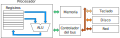
\includegraphics[scale=0.8]{img/sistema.pdf}
    \end{textblock}
    \begin{textblock}{140}(5,45)
    \begin{itemize}
%     \setlength\itemsep{0.5cm}
    \item<2-> El \textbf{Procesador} o CPU (\emph{Central Processing Unit}) es el encargado de tomar datos de la memoria o de dispositivos de entrada/salida, procesarlos y generar resultados o acciones sobre otros componentes del sistema.
    \item<3-> La \textbf{Memoria} se ocupa de almacenar datos para que puedan ser leídos o escritos por el procesador.
    \item<4-> Los \textbf{dispositivos de entrada/salida} nos permiten interactuar con el mundo exterior.
    \end{itemize}
    \end{textblock}
\end{frame}

\begin{frame}[fragile]{Sistema de Cómputo}
    Utilizando los circuitos que construimos hasta ahora vamos a armar un procesador.\\
    \bigskip
    La idea es \textbf{conectar componentes} entre sí, como registros y circuitos aritméticos, por medio de cables, a los que llamaremos buses.\\
    \bigskip
    Los \textbf{buses}, en esta primera aproximación, serán un conjunto ordenado de cables que nos permiten llevar datos desde un componente a otro.\\
    \bigskip
    Pero, \textbf{\textcolor{naranjauca}{¿cómo movemos datos de un componente a otro?}}
\end{frame}

\begin{frame}[fragile,t]{Transferencia entre registros}
    Supongamos dos registros bidireccionales conectados a un bus de 4 bits:\\
    \begin{center}
    \includegraphics[scale=0.7]{img/datapathDosRegistros-layer1.pdf} \hspace{1cm}
    \pause
    \includegraphics[scale=0.7]{img/datapathDosRegistros-layer2.pdf}
    \end{center}
    Este circuito puede ser representado como un \textbf{datapath}, donde se ilustra el camino que pueden hacer los datos entre los distintos componentes pasando por un bus.\\
    \bigskip
    \pause
    En este ejemplo, cada registro cuenta con dos señales:\\
    \begin{itemize}
    \setlength\itemsep{0cm}
    \item \normalsize \textbf{R}ead: {\small Si está en 1 presenta en el bus el dato almacenado en el registro.}\\
    \item \normalsize \textbf{W}rite: {\small Si está en 1 guarda en el registro el dato que esté en el bus.}\\
    \end{itemize}
    \begin{center}
    \textcolor{verdeuca}{Modificando el estado de las señales \textbf{R} y \textbf{W} de cada registro\\ buscamos copiar los datos entre ambos registros.}
    \end{center}
\end{frame}

\begin{frame}[fragile,t]{Transferencia entre registros}
    \begin{center}
    \includegraphics[scale=0.7]{img/datapathDosRegistros-layer2.pdf}
    \end{center}
    \pause
    \textcolor{gray}{\small {Copiar el dato almacenado en el Registro 0 al Registro 1:}}\\
    \begin{center} \footnotesize
    \begin{tabular}{|c|c|c|c|c|} \hline
     \texttt{clock}             & \texttt{reg0.R} & \texttt{reg0.W} & \texttt{reg1.R} & \texttt{reg1.W} \\ \hline
     {\tiny $\textifsym{h|l}$}  & \texttt{1}      & \texttt{0}      & \texttt{0}      & \texttt{1}      \\ \hline
    \end{tabular}
    \end{center}
    \pause
    \textcolor{gray}{\small {Copiar el dato almacenado en el Registro 1 al Registro 0:}}\\
    \begin{center} \footnotesize
    \begin{tabular}{|c|c|c|c|c|} \hline
     \texttt{clock}             & \texttt{reg0.R} & \texttt{reg0.W} & \texttt{reg1.R} & \texttt{reg1.W} \\ \hline
     {\tiny $\textifsym{h|l}$}  & \texttt{0}      & \texttt{1}      & \texttt{1}      & \texttt{0}      \\ \hline
    \end{tabular}
    \end{center}
    \normalsize
    Es decir, \textbf{modificando} las señales de los componentes podemos hacer \textbf{operaciones}.
\end{frame}

\begin{frame}[fragile,t]{Operaciones con registros}
    \footnotesize Supongamos el siguiente \emph{datapath}:
    \vspace{-0.05cm}
    \begin{center}
    \includegraphics[scale=0.7]{img/datapathRegistrosSumaAlu-layer1.pdf}
    \end{center}
    \pause
    \vspace{-0.5cm}
    \small 
    Agregamos dos registros denominados \texttt{A} y \texttt{B}, con solo una señal \textbf{W}.\\
    Los conectamos tal que el dato almacenado por ambos registros llegue a un sumador.\\
    La tarea del sumador es sumar los datos de ambos registros.\\
    Además, presenta el resultado en el bus si la señal de \textbf{en}able está en 1.\\
    \pause
    \begin{center}
    \normalsize \textcolor{naranjauca}{¿Cuál es la secuencia de operaciones para sumar los registros 0 y 1,\\ y guardar el resultado de la operación en el registro 0?}
    \end{center}
\end{frame}

\begin{frame}[fragile,t]{Operaciones con registros}
    \footnotesize Supongamos el siguiente \emph{datapath}:
    \vspace{-0.05cm}
    \begin{center}
    \includegraphics[scale=0.7]{img/datapathRegistrosSumaAlu-layer1.pdf}
    \end{center}
    \vspace{-0.5cm}
    \textcolor{gray}{\small {Sumar los datos almacenados en el Registro 0 y en el Registro 1, y guardar el resultado en el Registro 0:}}\\
    \begin{center} \footnotesize
    \begin{tabular}{|c|c|c|c|c|c|c|c|} \hline
     \texttt{clock}             & \texttt{reg0.R} & \texttt{reg0.W} & \texttt{reg1.R} & \texttt{reg1.W}  & \texttt{regA.W} & \texttt{regB.W} & \texttt{sum.en} \\ \hline \noalign{\pause}
     {\tiny $\textifsym{h|l}$}  & \texttt{1}      & \texttt{0}      & \texttt{0}      & \texttt{0}      & \texttt{1}       & \texttt{0}      & \texttt{0}      \\ \hline \noalign{\pause}
     {\tiny $\textifsym{h|l}$}  & \texttt{0}      & \texttt{0}      & \texttt{1}      & \texttt{0}      & \texttt{0}       & \texttt{1}      & \texttt{0}      \\ \hline \noalign{\pause} 
     {\tiny $\textifsym{h|l}$}  & \texttt{0}      & \texttt{1}      & \texttt{0}      & \texttt{0}      & \texttt{0}       & \texttt{0}      & \texttt{1}      \\ \hline
    \end{tabular}
    \end{center}
    \begin{center}
    \normalsize \textcolor{naranjauca}{¿Cómo hacer si queremos agregar más registros y hacer otras operaciones?}
    \end{center}
\end{frame}

\begin{frame}[fragile,t]{Operaciones con registros}
    \footnotesize Supongamos el siguiente \emph{datapath}:
    \vspace{-0.05cm}
    \begin{center}
    \includegraphics[scale=0.7]{img/datapathRegistrosSumaAlu-layer2.pdf}
    \end{center}
    \pause
    \small
    Para tener múltiples registros usamos un \emph{banco de registros}.\\ 
    Cuenta una señal que nos permite \textbf{seleccionar} el registro con el que buscamos operar.\\
    \bigskip
    Al sumador lo remplazamos por una \emph{ALU}, es decir, un circuito combinatorio que nos permite realizar distintas operaciones, tanto lógicas como aritméticas.\\
    \pause
    \begin{center}
    \normalsize \textcolor{naranjauca}{¿Qué secuencia de señales necesitamos para realizar\\ la operación anterior con este nuevo datapath?}
    \vspace{-1cm}
    \end{center}
\end{frame}

\begin{frame}[fragile,t]{Operaciones con registros}
    \footnotesize Supongamos el siguiente \emph{datapath}:
    \vspace{-0.05cm}
    \begin{center}
    \includegraphics[scale=0.7]{img/datapathRegistrosSumaAlu-layer2.pdf}
    \end{center}
    \textcolor{gray}{\small {Sumar los datos almacenados en el Registro 0 y en el Registro 1, y guardar el resultado en el Registro 0.s}}\\
    \begin{center} \footnotesize
    \begin{tabular}{|c|c|c|c|c|c|c|c|} \hline
                                & \multicolumn{3}{c|}{regBank} & \multicolumn{1}{c|}{regA} & \multicolumn{1}{c|}{regB} & \multicolumn{2}{c|}{ALU}\\ \hline
     \texttt{clock}             & \texttt{select} & \texttt{R} & \texttt{W} & \texttt{W} & \texttt{W} & \texttt{Operation} & \texttt{en} \\ \hline \noalign{\pause}
     {\tiny $\textifsym{h|l}$}  & \texttt{00}     & \texttt{1} & \texttt{0} & \texttt{1} & \texttt{0} & \texttt{}          & \texttt{0} \\ \hline \noalign{\pause}
     {\tiny $\textifsym{h|l}$}  & \texttt{01}     & \texttt{1} & \texttt{0} & \texttt{0} & \texttt{1} & \texttt{}          & \texttt{0} \\ \hline \noalign{\pause}
     {\tiny $\textifsym{h|l}$}  & \texttt{00}     & \texttt{0} & \texttt{1} & \texttt{0} & \texttt{0} & \texttt{+}         & \texttt{1} \\ \hline
    \end{tabular}
    \end{center}
\end{frame}

\begin{frame}[fragile,t]{Microarquitectura: Lenguaje y Notación}
    Para simplificar el estudio de los sistemas de cómputo, vamos a utilizar un lenguaje para expresar la transferencia entre registros.
    \begin{textblock}{70}(5,25)
    \begin{itemize}
    \setlength\itemsep{0.2cm}
    \item Definimos \textbf{componentes} como circuitos con entradas, salidas y señales.
    \item Las señales son entradas que modifican el \textbf{comportamiento} de los circuitos.
    \item Las señales se activan según como indique el \textbf{microprograma}.
    \item Estos serán listas de asignaciones entre registros y activación de señales que se realizan por cada ciclo de \textbf{clock}.
    \end{itemize}
    \end{textblock}
    \begin{textblock}{70}(80,18)
    \begin{center}
    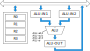
\includegraphics[scale=0.6]{img/datapathEjemploAlu.pdf}
    \end{center}
    \vspace{-0.3cm}
    \small
    \textcolor{gray}{Ejemplo:}
    Sumar el valor en el registro R0 con R1 y guardar el resultado en R0.\\
    \textcolor{verdeuca}{Microprograma}\\
    \vspace{-0.3cm}
    \begin{verbatim}
        ALU-IN1 := R0
        ALU-IN2 := R1
        ALU-add
        R0 := ALU-OUT
    \end{verbatim}
    \end{textblock}
\end{frame}

\begin{frame}[fragile,t]{Microarquitectura: Lenguaje y Notación}
    Supongamos el siguiente \emph{datapath}:
    \begin{textblock}{70}(8,20) \only<1->{ \includegraphics[scale=0.6]{img/datapathEjemploAluExtendida-layer1.pdf} } \end{textblock}
    \begin{textblock}{70}(8,20) \only<1->{ \includegraphics[scale=0.6]{img/datapathEjemploAluExtendida-layer2.pdf} } \end{textblock}
    \begin{textblock}{70}(8,20) \only<1->{ \includegraphics[scale=0.6]{img/datapathEjemploAluExtendida-layer3.pdf} } \end{textblock}
    \begin{textblock}{70}(8,20) \only<1->{ \includegraphics[scale=0.6]{img/datapathEjemploAluExtendida-layer4.pdf} } \end{textblock}
    \begin{textblock}{76}(70,18)
    \small
    Podemos además tener \textbf{otros componentes} con sus propias señales como \texttt{Incrementador} con las señales \texttt{INC+2} e \texttt{INC+1} y sus propios registros.\\
    \bigskip
    Pueden existir registros de \textbf{propósito específico} como PC o registros que proveen una constante como \texttt{0xFFFF}.\\
    \bigskip
    Podemos mover datos si hay un \textbf{camino directo} entre ellos.\\
    \scriptsize
    \begin{tabular}{l|c|l}
                & ¿vale?   & \\ \hline
    \texttt{R1 := R0   }   & \uncover<2->{\textcolor{green}{$\checkmark$}} & \uncover<2->{Copia \texttt{R0} en \texttt{R1}}\\
    \texttt{R0 := ALU-OUT} & \uncover<3->{\textcolor{green}{$\checkmark$}} & \uncover<3->{Copia \texttt{ALU-OUT} en \texttt{R0}}\\
    \texttt{R2 := 0xFFFF}  & \uncover<4->{\textcolor{green}{$\checkmark$}} & \uncover<4->{Copia la constante \texttt{0xFFFF} a \texttt{R2}}\\
    \texttt{ALU-OUT := R0} & \uncover<5->{\textcolor{red}{$\times$}}     & \uncover<5->{\texttt{ALU-OUT} es de solo lectura}\\
    \texttt{R0 := ALU-IN1} & \uncover<6->{\textcolor{red}{$\times$}}     & \uncover<6->{\texttt{ALU-IN1} es de solo escritura}\\
    \texttt{R1 := 0x35   } & \uncover<7->{\textcolor{red}{$\times$}}     & \uncover<7->{No se dispone de esa constante}\\
    \end{tabular}
    \end{textblock}
\end{frame}

\begin{frame}[fragile,t]{Microarquitectura: Lenguaje y Notación}
    Supongamos el siguiente \emph{datapath}:
    \begin{textblock}{70}(8,20) \only<1->{ \includegraphics[scale=0.6]{img/datapathEjemploAluExtendida-layer1.pdf} } \end{textblock}
    \begin{textblock}{70}(8,20) \only<1->{ \includegraphics[scale=0.6]{img/datapathEjemploAluExtendida-layer2.pdf} } \end{textblock}
    \begin{textblock}{70}(8,20) \only<1->{ \includegraphics[scale=0.6]{img/datapathEjemploAluExtendida-layer3.pdf} } \end{textblock}
    \begin{textblock}{70}(8,20) \only<1->{ \includegraphics[scale=0.6]{img/datapathEjemploAluExtendida-layer4.pdf} } \end{textblock}
    \begin{textblock}{70}(8,20) \only<1->{ \includegraphics[scale=0.6]{img/datapathEjemploAluExtendida-layer5.pdf} } \end{textblock}
    \begin{textblock}{70}(8,75) \scriptsize Todos los registros de 16 bits, excepto \texttt{Z} y \texttt{C} de 1 bit. \end{textblock}
    \begin{textblock}{76}(70,15)
    \small
    Todos los registros tienen un \textbf{tamaño}, al igual que los buses. No es posible asignar registros de distinto tamaño.\\
    \vspace{0.2cm}
    Sin embargo, podemos usar un solo bit de un registro para tomar decisiones.\\
    \vspace{0.2cm}
    \textcolor{gray}{Ejemplos:}\\
    \vspace{3.5cm}
    Para tomar múltiples bits es posible usar la notación de rangos, por ejemplo: \texttt{R0[3:0]}
    \end{textblock}
    \begin{textblock}{76}(70,45)
    \scriptsize
    \textcolor{verdeuca}{Microprograma 1}\\
    \vspace{-0.3cm}
    \begin{verbatim}
    if ALU_OUT[15] = 1
        INC-IN := PC
        INC+2
        PC := INC-OUT
    else
        INC-IN := PC
        INC+1
        PC := INC-OUT
    \end{verbatim}
    \end{textblock}
    \begin{textblock}{76}(110,45)
    \scriptsize
    \textcolor{verdeuca}{Microprograma 2}\\
    \vspace{-0.3cm}
    \begin{verbatim}
    if Z = 1
        INC-IN := PC
        INC+2
        PC := INC-OUT
    else
        INC-IN := PC
        INC+1
        PC := INC-OUT
    \end{verbatim}
    \end{textblock}
\end{frame}

\begin{frame}[fragile,t]{Unidad de Control}
    Existe un componente más dentro del \textbf{datapath} encargado de modificar el valor de las señales de los distintos componentes para realizar alguna acción.\\
    \bigskip
    Este componente se denomina \textbf{Unidad de Control}.\\
    \bigskip
    \pause
    Funciona como un \textbf{secuenciador}: una vez identificada la tarea a realizar, genera una secuencia de señales (\emph{microinstrucciones}) para realizar la acción correspondiente.\\
    Esta secuencia de señales la podemos suponer fija y almacenada dentro de una memoria.\\
    \begin{center}
    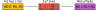
\includegraphics[scale=0.8]{img/secuenciador.pdf}
    \end{center}
    A cada \textbf{instrucción} le corresponde una secuencia de señales.\\
    El proceso para convertir una instrucción en una secuencia de señales\\
    se denomina \textbf{decodificación}.
\end{frame}

\begin{frame}[fragile,t]{Ciclo de Instrucción}
    Los programas son secuencias de \textbf{instrucciones} que los procesadores pueden\\ interpretar y ejecutar.
    Pero, \textcolor{naranjauca}{¿cómo hacen esta tarea?}\\
    \vspace{0.2cm}
    \only<2->{Realizan tres pasos todo el tiempo por cada instrucción a ejecutar.}
    \begin{textblock}{100}(10,36)
    \only<2->{ 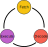
\includegraphics[scale=0.7]{img/fetchDecodeExecute.pdf} }
    \end{textblock}
    \begin{textblock}{100}(50,30)
    \begin{itemize}
    \small \setlength\itemsep{0.3cm}
    \item<2-> \textbf{Fetch}:
    Lectura desde la memoria de la instrucción a ejecutar.
    Esta puede ser de tamaño fijo o de tamaño variable.
    \item<3-> \textbf{Decode}:
    Se interpreta la instrucción, identificando la acción que debe ser realizada (opcode) y los operandos.
    Puede ser necesario hacer múltiples accesos a memoria para cargar los operandos a registros.
    \item<4-> \textbf{Execute}:
    Se ejecuta la operación. Puede ser una operación aritmética o lógica, un acceso a memoria o movimiento entre registros, incluso la configuración de algún registro dentro del procesador.
    \end{itemize}
    \end{textblock}
    \begin{textblock}{100}(10,80)
    \only<5->{ Pero, \textcolor{naranjauca}{\textbf{¿cuál es la próxima instrucción a ejecutar?}} }
    \end{textblock}
\end{frame}

\begin{frame}[fragile,t]{Program Counter}
    Los procesadores poseen un registro especial denominado \textbf{Program Counter} o \textbf{PC}.\\
    \vspace{0.1cm}
    Este registro guarda una dirección de \textbf{memoria}.
    \pause
%     \vspace{0.2cm}
    \begin{block}{Memoria}
    \small
    La memoria es el componente que nos permite almacenar programas y datos.
    Está organizada para ser accedida mediante direcciones. Una dirección de memoria identifica una unidad direccionable de un tamaño fijo. Por ejemplo, 1 byte.
    \end{block}
    \textcolor{gray}{Ejemplo:}
    \begin{center}
    \vspace{1.1cm}
    \footnotesize Memoria direccionable a byte, es decir, cada dirección de memoria apunta a un byte.\\
    \end{center}
    \uncover<3->{El PC apunta a la dirección \texttt{0x20A0}, donde se encuentra almacenado el valor \texttt{01001001b}.\\}
    \uncover<4->{Si cada instrucción ocupa 2 bytes,} \uncover<5->{la próxima instrucción a ejecutar es \texttt{0x20A2}.\\}
    \uncover<6->{Y ahora, \textcolor{naranjauca}{\textbf{¿cómo leemos instrucciones?}}}
    \begin{textblock}{70}(21.2,48.7) \only<2->{ \includegraphics[scale=1.2]{img/programCounter-layer1.pdf} } \end{textblock}
    \begin{textblock}{70}(21.2,48.7) \only<3-4>{\includegraphics[scale=1.2]{img/programCounter-layer2.pdf} } \end{textblock}
    \begin{textblock}{70}(21.2,48.7) \only<4-4>{\includegraphics[scale=1.2]{img/programCounter-layer3.pdf} } \end{textblock}
    \begin{textblock}{70}(21.2,48.7) \only<5-|handout:0>{ \includegraphics[scale=1.2]{img/programCounter-layer4.pdf} } \end{textblock}
    \begin{textblock}{70}(21.2,48.7) \only<5-|handout:0>{ \includegraphics[scale=1.2]{img/programCounter-layer5.pdf} } \end{textblock}
\end{frame}

\begin{frame}[fragile,t]{Componente de memoria}
    Supongamos el siguiente \emph{datapath}:\\
    \vspace{6.6cm}
    \uncover<5->{Y ahora, \textcolor{naranjauca}{\textbf{¿cómo escribimos instrucciones?}}}
    \begin{textblock}{70}(5,18) \only<1->{ 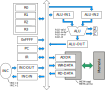
\includegraphics[scale=0.6]{img/datapathEjemploAluCompleta.pdf} } \end{textblock}
    \begin{textblock}{70}(8,76) \scriptsize Todos los registros de 16 bits, excepto \texttt{Z} y \texttt{C} de 1 bit. \end{textblock}
    \begin{textblock}{76}(75,8)
    \small
    La \textbf{interfaz} con la memoria la vamos a modelar como un dispositivo más, que se conecta mediante un \textbf{bus externo} a la memoria.\\
    \vspace{0.2cm}
    \footnotesize
    \uncover<2->{
    Para acceder a la memoria tenemos tres registros:\\    
    \hspace{0.3cm}\textbf{ADDR}: Contiene la dirección a leer o escribir.\\
    \hspace{0.3cm}\textbf{WR-DATA}: Contiene el dato a escribir en memoria. \\
    \hspace{0.3cm}\textbf{RD-DATA}: Contiene el dato leído de memoria.\\
    \vspace{0.2cm}
    } \uncover<3->{
    Y contamos con dos señales.\\
    \hspace{0.3cm}\textbf{MEM-read}: Lee un dato de la dirección \texttt{ADDR} y\\ \hspace{1.8cm} copia su contenido en \texttt{RD-DATA}.\\
    \hspace{0.3cm}\textbf{MEM-write}: Escribe el dato \texttt{WR-DATA} en la dirección \texttt{ADDR}.\\
    \vspace{0.3cm}
    } \uncover<4->{
    \textcolor{gray}{Ejemplos:}\\ }
    \end{textblock}
    \begin{textblock}{76}(80,65)
    \only<4->{
    \scriptsize
    \textcolor{verdeuca}{Microprograma 1}\\
    \texttt{ADDR := PC}\\
    \texttt{MEM-read}\\
    \texttt{IR := RD-DATA}\\
    }
    \end{textblock}
    \begin{textblock}{76}(120,65)
    \only<4->{
    \scriptsize
    \textcolor{verdeuca}{Microprograma 2}\\
    \texttt{ADDR := R0}\\
    \texttt{WR-DATA := R1}\\
    \texttt{MEM-write}\\
    }
    \end{textblock}
\end{frame}

\begin{frame}[fragile,t]{Lenguaje ensamblador}
    Llamamos \textbf{lenguaje de máquina} al conjunto de instrucciones que el procesador puede interpretar y ejecutar. \\
    Llamamos \textbf{lenguaje ensamblador} a las instrucciones del lenguaje de máquina escritas como texto.\\
    \bigskip
    \pause
    Las instrucciones en lenguaje ensamblador se deben traducir a instrucciones en lenguaje de máquina.
    La aplicación encargada de hacer esta traducción se denomina \textbf{ensamblador}.\\
    \begin{center}
    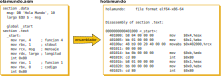
\includegraphics[scale=0.57]{img/ensamblador.pdf} 
    \end{center}
\end{frame}

\begin{frame}[fragile,t]{Organización vs Arquitectura}
    \begin{textblock}{70}(10,20)
    \large \textcolor{naranjauca}{\textbf{Arquitectura}}\\ \vspace{0.5cm}
    \normalsize
    \only<2->{
    Componentes \textbf{visibles} al programador.\\
    \begin{itemize}
    \setlength\itemsep{0.2cm}
    \item Identificación de registros.
    \item Conjunto de instrucciones\\ (\emph{Instruction Set Architecture}).
    \item Modos de acceso a memoria.
    \item Mecanismos de entrada/salida.
    \end{itemize}
    }
    \end{textblock}
    \begin{textblock}{70}(85,20)
    \large \textcolor{naranjauca}{\textbf{Organización}}\\ \vspace{0.5cm}
    \normalsize
    \only<3->{
    \textbf{Implementación} de una arquitectura.\\
    \begin{itemize}
    \setlength\itemsep{0.2cm}
    \item Señales de la unidad de control.
    \item Implementación de microinstrucciones\\ o hardware específico.
    \item Cantidad y uso de unidades funcionales.
    \item Tecnología de integración.
    \end{itemize}
    }
    \end{textblock}
    \begin{textblock}{140}(10,68)
    \only<4->{
    \begin{center}
    \textcolor{verdeuca}{Hasta el momento, estudiamos la \textbf{organización} de un sistema de computo.\\
    Ahora vamos a estudiar su \textbf{arquitectura}.}
    \end{center}
    }
    \end{textblock}
\end{frame}

\begin{frame}[fragile,t]{Arquitectura OrgaSmall}
    \small
    Para ilustrar el funcionamiento de un sistema de computo, vamos a presentar la arquitectura \emph{OrgaSmall}.\\
    \vspace{0.2cm}
    Esta arquitectura fue diseñada con fines didácticos y su objetivo es poner de manifiesto todos los conceptos básicos de la organización de un procesador con una arquitectura simple.\\
    \bigskip    
    \begin{textblock}{100}(10,30)
    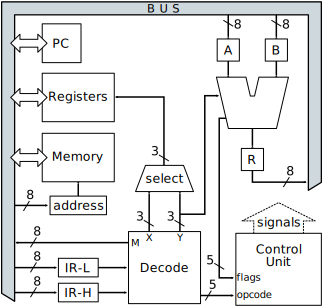
\includegraphics[scale=0.6]{img/arquitectura_micro.pdf}
    \end{textblock}
    \begin{textblock}{100}(70,30)
    \begin{itemize}
    \item 8 registros de propósito general, \texttt{R0} a \texttt{R7}.
    \item 1 registro de propósito específico PC.
    \item Unidad direccionable de 8 bits (1 byte) e \\ instrucciones de 16 bits (2 bytes).
    \item Memoria de 256 bytes.
    \item Bus de 8 bits.
    \item Diseño microprogramado.
    \end{itemize}
    \end{textblock}
\end{frame}

\begin{frame}[fragile]
    \frametitle{Bibliografía}
    \begin{itemize}
     \setlength\itemsep{0.5cm}
    \item[-] \small Tanenbaum, “Organización de Computadoras. Un Enfoque Estructurado”, 4ta Edición, 2000.\\
    \begin{itemize}
     \item \textbf{Capítulo 2 - Organización de los Sistemas de Computadora} - Páginas 39-45
     \item \textbf{Capítulo 4 - El nivel de Microarquitectura} - Páginas 203-215
    \end{itemize}
    \item[-] \small Null, “Essentials of Computer Organization and Architecture”, 5th Edition, 2018.\\
    \begin{itemize}
     \item \textbf{Chapter 4 - MARIE: An Introduction to a Simple Computer}
     \begin{itemize}
     \item 4.2 CPU Basics and Organization
     \item 4.3 The Bus
     \item 4.6 Memory Organization and Adressing
     \item 4.8 MARIE
     \item 4.9 Instruction Processing
     \end{itemize}
    \end{itemize}
%     \item[-] \small Silberschatz, “Fundamentos de Sistemas Operativos”, 7ma Edición, 2006.\\
%     \item[-] \small Tanenbaum, “Modern Operating Systems”, 4th Edition, 2015.\\
    \end{itemize}
     \textcolor{naranjauca}{Referencias}
     \begin{itemize}
    \item[-] Especificación de la Arquitectura OrgaSmall\\ \small \url{https://github.com/fokerman/microOrgaSmall/}
    \end{itemize}
\end{frame}

% \begin{frame}[fragile]
%     \frametitle{Ejercicios}
%     Con lo visto, ya pueden resolver todos los ejercicios de la Guía de Lógica Digital.
% \end{frame}

\begin{frame}[plain]
    \begin{center}
    \vspace{2cm}
    \huge ¡Gracias!\\
    \vspace{2cm}
%     \normalsize Recuerden leer los comentarios adjuntos\\ en cada clase por aclaraciones.
    \end{center}
\end{frame}

\end{document}
